\subsection{Seconda parte - impatto dei parametri \texorpdfstring{$F$}{F} e \texorpdfstring{$D$}{D} }

Il progetto offre la possibilità di scegliere finestre di grandezza variabile per l'applicazione delle funzioni dct2/idct2, questo avviene tramite la scelta di un opportuno parametro F, rappresentante la dimensione dei blocchi a cui applicare la conversione; e l'implementazione della funzionalità di compressione (taglio dei coefficienti della funzione) tramite la scelta di opportuno parametro $d$ rappresenta una soglia di taglio sulle frequenze: vengono mantenuti solo i coefficienti $c_{k,\ell}$ tali che $k + \ell < d$.

\subsection*{Scelta di \texorpdfstring{$F$}}
\begin{itemize}
  \item Un valore piccolo di $F$ (ad esempio 4 o 8) porta ad una maggiore granularità. Questo comporta un numero elevato di blocchi, producendo un'immagine che risulta più dettagliata all'occhio umano, e permette di ridurre la dimensione del talio ai bordi delle immagini.
  \item Un valore grande di $F$ (come 32 o 64) riduce il numero di trasformate da calcolare, ma include porzioni di immagine più eterogenee in ciascun blocco, riducendo l'efficacia della compressione e la qualità del risultato.
\end{itemize}

\begin{figure}[H]
    \centering
    \begin{subfigure}[b]{0.49\textwidth}
        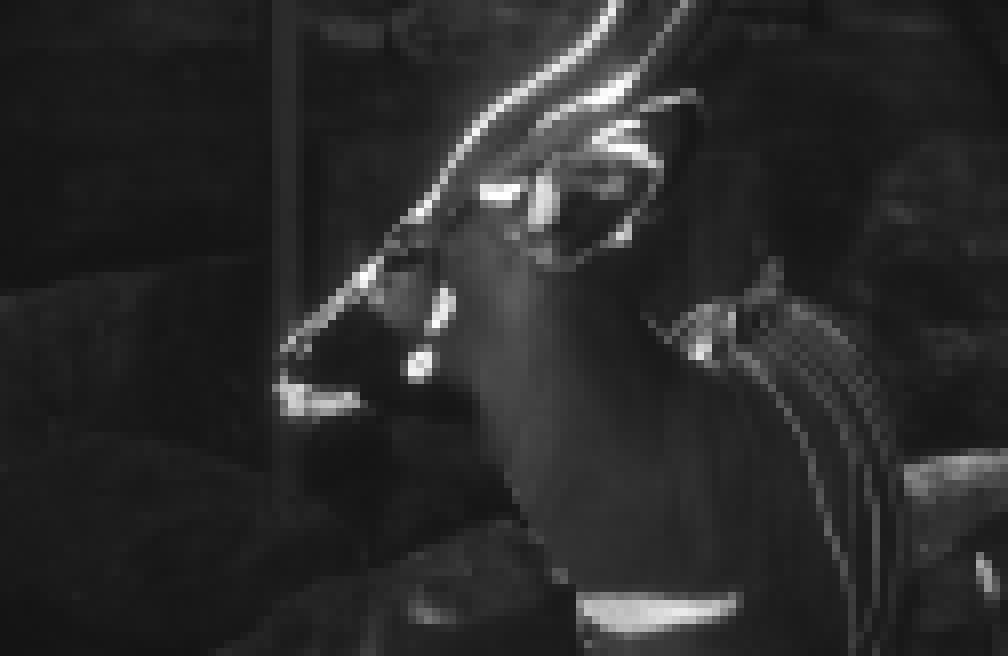
\includegraphics[width=\textwidth]{images/f/f8_d1.jpg}
        \caption{f = 8}
    \end{subfigure}
    \hfill
    \begin{subfigure}[b]{0.49\textwidth}
        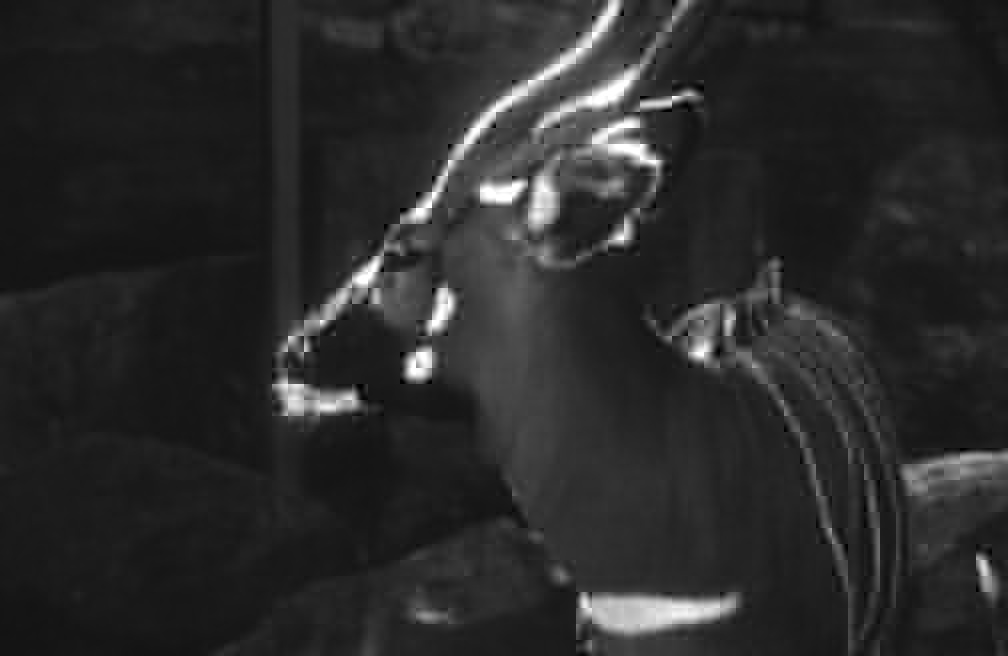
\includegraphics[width=\textwidth]{images/f/f16_d3.jpg}
        \caption{f = 16}
    \end{subfigure}

    \vspace{0.2cm}

    \begin{subfigure}[b]{0.49\textwidth}
        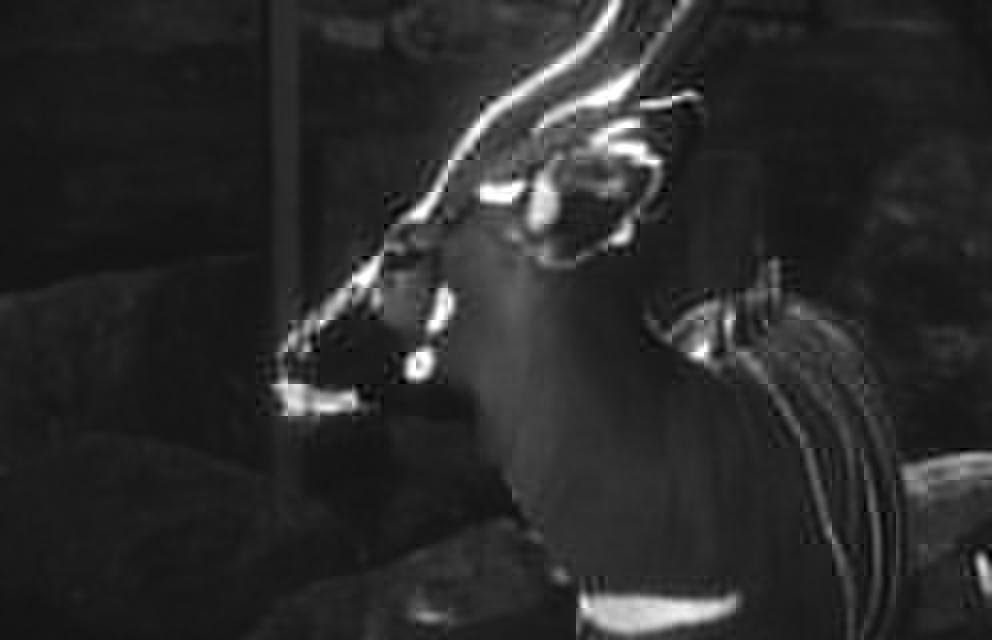
\includegraphics[width=\textwidth]{images/f/f32_d6.jpg}
        \caption{f = 32}
    \end{subfigure}
    \hfill
    \begin{subfigure}[b]{0.49\textwidth}
        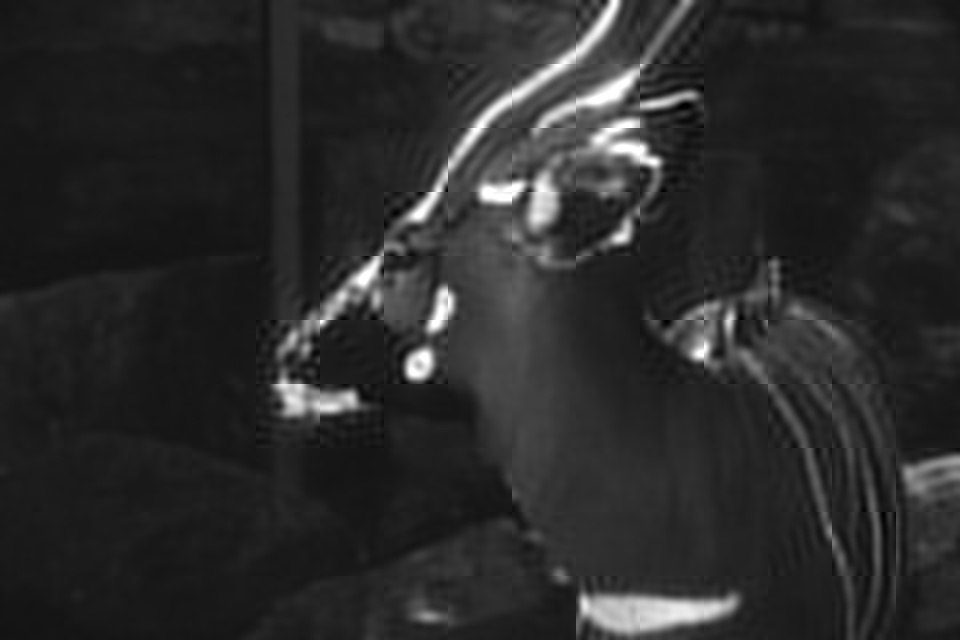
\includegraphics[width=\textwidth]{images/f/f64_d12.jpg}
        \caption{f = 64}
    \end{subfigure}
    \label{fig:griglia}
\end{figure}

\subsection*{Scelta di \texorpdfstring{$d$}}
\begin{itemize}
  \item Un valore basso di $d$ implica un taglio più severo delle componenti in frequenza: vengono eliminate più frequenze, l'implementazione di un parametro d come quella proposta in questo progetto non permette di discriminare tra frequenze che hanno più peso nel determinare i dettagli di un'immagine; vengono quindi sempre eliminate le frequenze più alte, indiscriminatamete.
  \item Un valore alto di $d$ preserva una maggiore quantità di informazione, vengono tagliati meno coefficienti, risultando in un’immagine più fedele all’originale.
  
\end{itemize}
\begin{figure}[h]
    \centering
    \begin{subfigure}[b]{0.45\textwidth}
        
\includegraphics[width=\textwidth]{images/d/d4_f64.jpg}
        \caption{d = 4}
    \end{subfigure}
    \hfill
    \begin{subfigure}[b]{0.45\textwidth}
        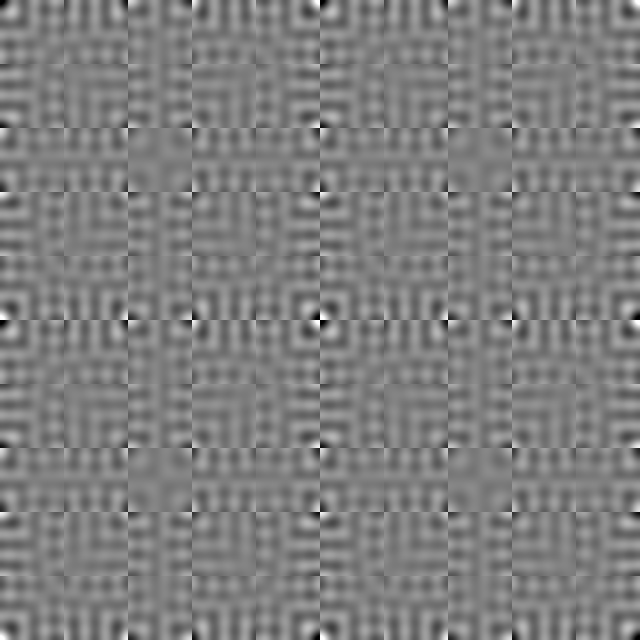
\includegraphics[width=\textwidth]{images/d/d8_f64.jpg}
        \caption{d = 8}
    \end{subfigure}

    \vspace{0.2cm}

    \begin{subfigure}[b]{0.45\textwidth}
        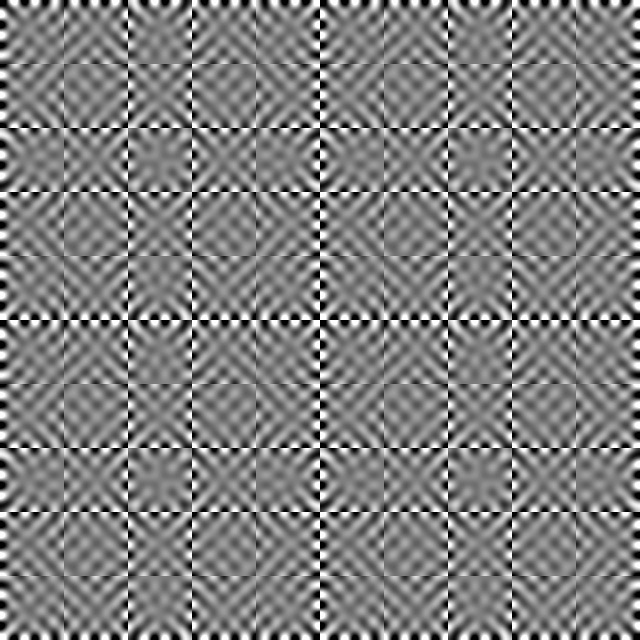
\includegraphics[width=\textwidth]{images/d/d12_f64.jpg}
        \caption{d = 12}
    \end{subfigure}
    \hfill
    \begin{subfigure}[b]{0.45\textwidth}
        
\includegraphics[width=\textwidth]{images/d/d16_f64.jpg}
        \caption{d = 16}
    \end{subfigure}
    \label{fig:griglia}
\end{figure}

